\subsection*{Task 1}

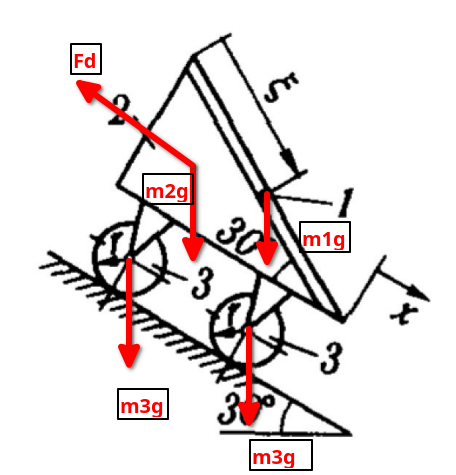
\includegraphics[height=8cm]{task1.png}

\begin{enumerate}
    \item RO: system of pulley, two masses
    \item Motion: A, B - rectilinear
    \item Conditions: \\
          \begin{tabular}{|c|c|c|}
              \hline
              $$    & $initial$ & $final$ \\
              \hline
              $y_A$ & $y_A^0$   & $?$     \\
              \hline
              $y_B$ & $y_B^0$   & $?$     \\
              \hline
              $v_A$ & $0$       & $v + a$ \\
              \hline
              $v_B$ & $0$       & $-v$    \\
              \hline
              $a_A$ & $-g$      & $-g$    \\
              \hline
              $a_B$ & $-g$      & $-g$    \\
              \hline
          \end{tabular}
    \item Force analysis: \\
          $m_A\vec{g}$, $m_B\vec{g}$, $m_{pulley}\vec{g}$, $\vec{R}$
    \item Method: Theorem of change of angular momentum of the system
    \item Solution:
          \begin{enumerate}
              \item Find momentum around axis $z$:
                    \begin{align}
                        -m_ag \cdot r + m_bg \cdot r = 0
                    \end{align}
                    We know that $\sum M_z(\vec{F}_i) = 0$ which makes easier to use the theorem.
              \item Theorem application:
                    \begin{align}
                        0 = L_{pulley} + L_{A} + L_{B} \\
                        0 = I\omega + m \cdot v_a \cdot r + m \cdot v_b \cdot r \\
                        0 = \frac{m r^2}{4}(\frac{v_b}{r}) + m \cdot (v_b + a) \cdot r + m \cdot v_b \cdot r
                    \end{align}

          \end{enumerate}
          \item Answer:
          \begin{answer}
              \begin{align}
                  v_b = - \frac{4 \cdot a}{9} \notag
              \end{align}
              mass B will start to move upwards
          \end{answer}
\end{enumerate}